% \documentclass{article} uncomment to compile in overleaf
\usepackage{graphicx}
\usepackage{tabularx}
\usepackage{amsmath}
\usepackage[T2A]{fontenc}
\usepackage[top=5cm,bottom=3cm,right=3cm,left=3cm]{geometry}
\usepackage[utf8]{inputenc}

\title{Анализ программ - Lab2}
\author{Матвей Русаков m.rusakov@innopolis.university SD-03}
\date{Апрель 2025}

\begin{document}

    \maketitle


    \section*{Предисловие}

    Материал и скриншоты из гидры я разместил на GitHub, в директории Lab2/lab\_data/ вы можете найти исходник,
    скриншоты и сишный код мейн функции для каждой из задач

    \section*{Task 0}
    \paragraph{Мейн функция} нулевой задачи выглядит вот так:

\begin{verbatim}
undefined8 FUN_00101170(void)

{
  int iVar1;
  char *__s1;

  __s1 = (char *)malloc(400);
  printf("%s","Hello, enter the flag:\n");
  __isoc99_scanf(&DAT_00102004,__s1);
  iVar1 = strcmp(__s1,"flag{6057f13c496ecf7fd777ceb9e79ae2 85}");
  if (iVar1 == 0) {
    printf("%s",&DAT_00102046);
  }
  else {
    printf("%s","TRY HARDER");
  }
  return 0;
}

\end{verbatim}

\paragraph{Описание}

\paragraph{}
Данный код --- это функция на языке C, реализующая проверку флага.
Опишем её по шагам:

\begin{enumerate}
    \item Выделяется память под строку:
    \begin{verbatim}
    __s1 = (char *)malloc(400);
    \end{verbatim}
    Здесь выделяются 400 байт для хранения пользовательского ввода.

    \item Печатается приглашение пользователю:
    \begin{verbatim}
    printf("%s", "Hello, enter the flag:\n");
    \end{verbatim}
    На экран выводится сообщение:
    \begin{verbatim}
    Hello, enter the flag:
    \end{verbatim}

    \item Считывается ввод:
    \begin{verbatim}
    __isoc99_scanf(&DAT_00102004, __s1);
    \end{verbatim}

    \item Введённая строка сравнивается с жёстко закодированным флагом:
    \begin{verbatim}
    iVar1 = strcmp(__s1, "flag{6057f13c496ecf7fd777ceb9e79ae285}");
    \end{verbatim}
    Если строки совпадают (iVar1 == 0), выполняется блок if, иначе --- else.

    \item Условие:
    \begin{verbatim}
    if (iVar1 == 0)
        printf("%s", &DAT_00102046);
    else
        printf("%s", "TRY HARDER");
    \end{verbatim}
    Если строка верная, выводится сообщение по адресу \&DAT\_00102046 (строка \("\)WIN\("\)), иначе выводится сообщение \("\)TRY HARDER\("\).

    \item Функция возвращает 0:
    \begin{verbatim}
    return 0;
    \end{verbatim}
\end{enumerate}

\noindent

\paragraph{Особенности}
\begin{itemize}
    \item Отсутствует освобождение памяти после \texttt{malloc} (утечка памяти);
    \item Формат ввода не позволяет вводить пробелы (если используется \%s);
    \item Сравнение производится напрямую, без шифрования или дополнительных преобразований.
\end{itemize}

\newpage

\paragraph{Тестовые запуски}

\paragraph{}
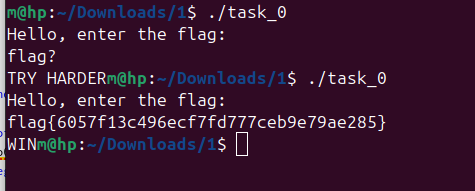
\includegraphics[width=0.7\linewidth]{static/solution_task_0}


    \section*{Task 1}
    \paragraph{Как выглядит мейн функция} - вы можете найти на гитхабе в референсах.
Она слишком длинная, чтобы записывать ее в репорт

\paragraph{Описание}

Данный код --- это функция на языке C, которая реализует проверку флага, аналогичную предыдущей, но с поэтапной посимвольной проверкой.
Опишем её по шагам:

\begin{enumerate}
    \item Объявление локальных переменных и инициализация:
    \begin{verbatim}
    int iVar1;
    int local_40;
    int local_3c;
    char local_38 [4];
    char cStack_34;
    char cStack_33;
    ...
    char acStack_13 [7];
    undefined4 local_c;

    local_c = 0;
    local_3c = 0;
    \end{verbatim}

    \item Приветственное сообщение:
    \begin{verbatim}
    printf("%s",
      "Hello, this task is very similar to the
      previous one, but has  some
      modifications\nenter the flag:\n"
    );
    \end{verbatim}
    Выводит сообщение с просьбой ввести флаг.

    \item Чтение посимвольного ввода (38 символов):
    \begin{verbatim}
    for (local_40 = 0; local_40 < 0x26; local_40 = local_40 + 1) {
      __isoc99_scanf(&DAT_00102069, local_38 + local_40);
    }
    \end{verbatim}

    \item Пошаговое посимвольное сравнение (каждый символ сравнивается отдельно через \texttt{strncmp}), например:
    \begin{verbatim}
    iVar1 = strncmp("f", local_38, 1);
    if (iVar1 == 0) {
      local_3c = 1;
      iVar1 = strncmp("l", local_38 + 1, 1);
      if (iVar1 == 0) {
        local_3c = 2;
        iVar1 = strncmp("a", local_38 + 2, 1);
        if (iVar1 == 0) {
          local_3c = 3;
          ...
    \end{verbatim}

    Проверка продолжается символ за символом:
    \begin{verbatim}
    ...
    iVar1 = strncmp("}", acStack_13, 1);
    if (iVar1 == 0) {
      local_3c = 0x26;
    }
    \end{verbatim}

    \item Финальная проверка:
    \begin{verbatim}
    if (local_3c == 0x26) {
      printf("%s", &DAT_00102097);
    }
    else {
      printf("%s", "TRY HARDER");
    }
    \end{verbatim}

    \item Возврат из функции:
    \begin{verbatim}
    return 0;
    \end{verbatim}
\end{enumerate}

\paragraph{Отличия и особенности}
\begin{itemize}
    \item task\_0 считывает строчку - после enter или пробела запустится скрипт дальше, в то время как в task\_1 используется посимвольный ввод

    \item Поскольку флаг состоит из 38 символов, функция будет ждать, пока пользователь не введет 38 символов и только потом запустит дальше

    \item В task\_1 последовательное, посимвольное сравнение с буквами из правильного флага

    \item Флаг для этой задачи немного другой - flag\{444Y0urB4seRBe803g2Usdfd4ds9y1re\}
\end{itemize}

\paragraph{Тестовые запуски}

\paragraph{}

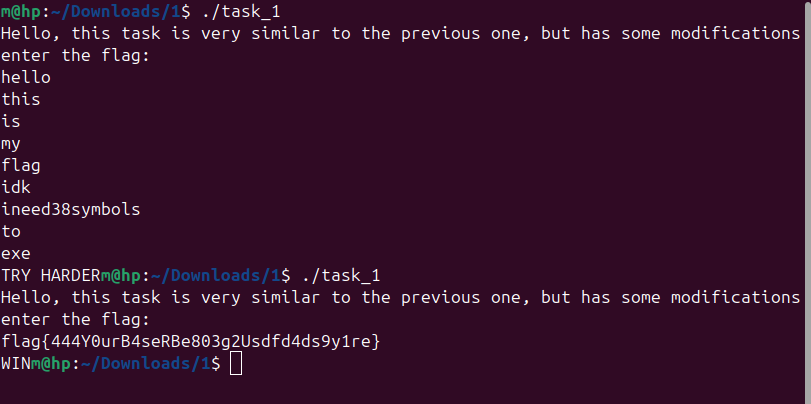
\includegraphics[width=0.75\linewidth]{static/solution_task_1}


    \section*{Task 2}
    \paragraph{Мейн}
В этой задаче исходный код функции отсутствует, программа не запускается, но есть информация, которую можно посмотреть в ghidra

\paragraph{Описание}
\begin{enumerate}
    \item Попытка запуска исполняемого файла без прав:
    \begin{verbatim}
    m@hp:~/Downloads/1$ ./task_2
    bash: ./task_2: Permission denied
    \end{verbatim}
    Вывод: нет прав на выполнение файла.

    \item Попытка запуска через \texttt{sudo}:
    \begin{verbatim}
    m@hp:~/Downloads/1$ sudo ./task_2
    [sudo] password for m:
    sudo: ./task_2: command not found
    \end{verbatim}
    Вывод: несмотря на \texttt{sudo}, команда не найдена.
    Файл не является исполняемым бинарником.
    Далее я посмотрел информацию о файле внутри ghidra, а также попробовал вывести все строчки с помощью команды \texttt{strings}
    \item Просмотр строк внутри файла через \texttt{strings}:
    \begin{verbatim}
    m@hp:~/Downloads/1$ strings task_2
    Linux
    Linux
    1Hello!
    1Bye-bye :(
    license=flag{baee49fd4f7009ff6e932463791f28e6}
    srcversion=FED0633F3F673540E886029
    depends=
    retpoline=Y
    name=task_7
    vermagic=6.2.0-34-generic SMP preempt mod_unload modversions
    __fentry__
    _printk
    __x86_return_thunk
    module_layout
    task_7
    GCC: (Ubuntu 11.4.0-1ubuntu1~22.04) 11.4.0
    GCC: (Ubuntu 11.4.0-1ubuntu1~22.04) 11.4.0
    .shstrtab
    .note.gnu.build-id
    .note.Linux
    .text
    .rodata.str1.1
    __mcount_loc
    .modinfo
    .return_sites
    .call_sites
    __versions
    __patchable_function_entries
    .exit.data
    .init.data
    .gnu.linkonce.this_module
    .bss
    .comment
    .note.GNU-stack
    \end{verbatim}

    \item Ключевой момент — найденная строка:
    \begin{verbatim}
    license=flag{baee49fd4f7009ff6e932463791f28e6}
    \end{verbatim}
\end{enumerate}

\vspace{0.5cm}

\noindent

\paragraph{Особенности}
\begin{itemize}
    \item Файл \texttt{task\_2} не является обычным исполняемым файлом, а представляет собой скомпилированный модуль ядра Linux.
    \item Запуск напрямую не работает, потому что модуль нужно загружать через \texttt{insmod} или \texttt{modprobe}, а не исполнять.
    \item Флаг хранится в строке с \texttt{license} внутри модуля.
    \item Флаг: flag\{baee49fd4f7009ff6e932463791f28e6\}
    \item В выводе присутсвует \("\)depends= \ldotsname=task\_7\ldots\("\), возможно этот файл содержит выводы для
    7го задания типа \("\)Hello!\("\) и \("\)Bye-bye :$($\("\).
    ФФлаг, найденный здесь, возможно, подойдет для решения 7й задачи.
\end{itemize}

\paragraph{Тестовые запуски} были в описании, поэтому прикреплю скриншот из гидры с полем лицензии и флага

\paragraph{}
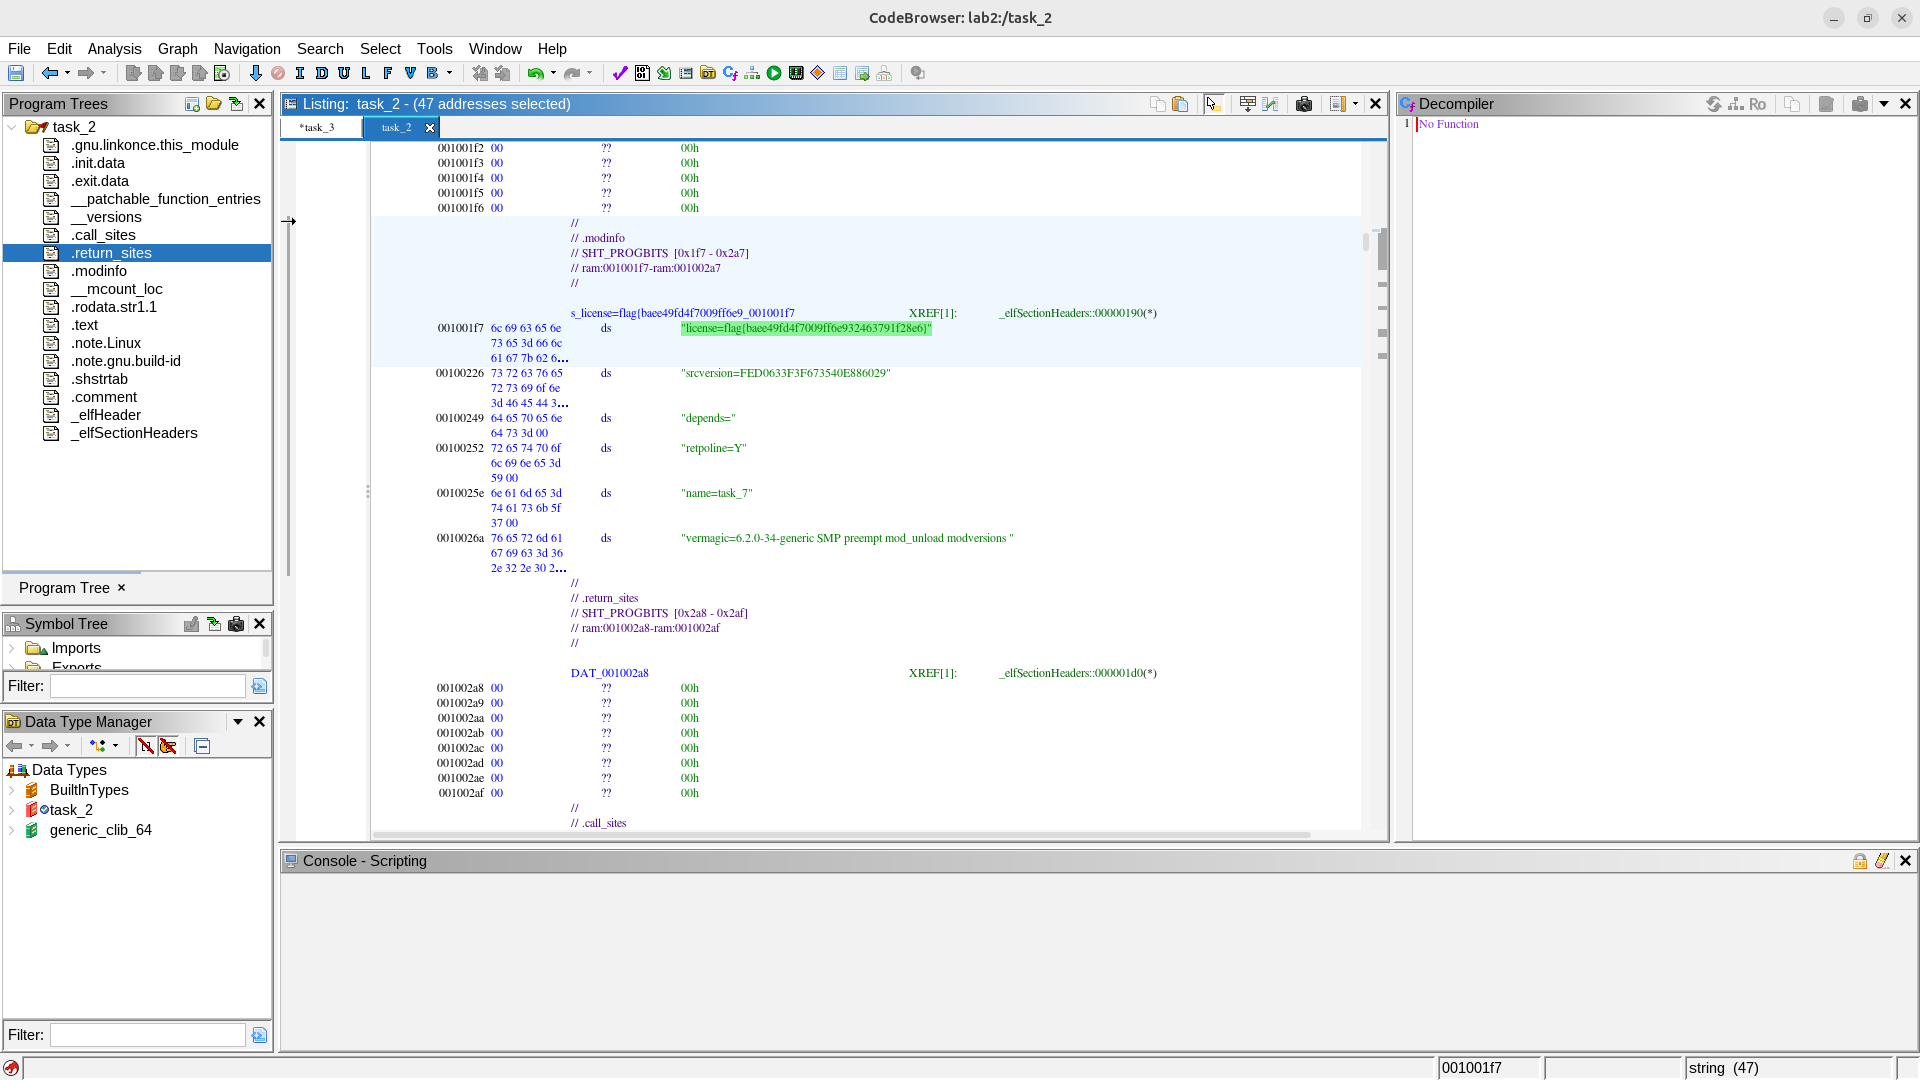
\includegraphics[width=1\linewidth]{static/solution_task_2}


    \section*{Task 3}
    \paragraph{Мейн}
В этой задаче мы снова имеем дело с модулем ядра, который не запускается напрямую как исполняемый файл, но доступен для анализа через вывод команды \texttt{strings} и в ghidra.

\paragraph{Описание}
\begin{enumerate}
    \item Попытка запуска файла с правами суперпользователя:
    \begin{verbatim}
    m@hp:~/Downloads/1$ sudo ./task_3
    [sudo] password for m:
    sudo: ./task_3: command not found
    \end{verbatim}
    Вывод: команда не найдена. Скорее всего, файл не является исполняемым бинарником, а модулем ядра.

    \item Просмотр строк в файле через \texttt{strings}:
    \begin{verbatim}
    m@hp:~/Downloads/1$ strings task_3
    Linux
    Linux
    AUATI
    A]A^]1
    flag
    itmo
    6[*] Bye - bye !
    1reading...
    1[*] Error assigning Major Number!
    1[*] Failed to register device class
    1[*] Failed to create the device
    G'g/|
    W[0sd
    q-fn
    rEdWcNDyavDSNOdKOC95iTEP8bioF3IPmAKUXx
    license=GPL
    description=find the flag
    srcversion=0765CAD67B0F0DF80A62408
    depends=
    retpoline=Y
    name=task_8
    vermagic=6.2.0-34-generic SMP preempt mod_unload modversions
    __register_chrdev
    __class_create
    device_create
    __x86_return_thunk
    _printk
    class_destroy
    __unregister_chrdev
    device_destroy
    class_unregister
    vmalloc
    __check_object_size
    _copy_to_user
    __copy_overflow
    __fentry__
    module_layout
    task_8
    GCC: (Ubuntu 11.4.0-1ubuntu1~22.04) 11.4.0
    GCC: (Ubuntu 11.4.0-1ubuntu1~22.04) 11.4.0
    __UNIQUE_ID_srcversion193
    __UNIQUE_ID_depends192
    ____versions
    __UNIQUE_ID_retpoline191
    __UNIQUE_ID_name190
    __UNIQUE_ID_vermagic189
    _note_10
    _note_9
    intro_init
    fops
    __key.11
    my_class
    intro_exit
    __UNIQUE_ID___addressable_cleanup_module241
    __UNIQUE_ID___addressable_init_module240
    __UNIQUE_ID_license239
    __UNIQUE_ID_description238
    __pfx_intro_read
    __check_object_size
    __class_create
    __this_module
    class_destroy
    crypted
    __fentry__
    _printk
    __copy_overflow
    __pfx_init_module
    major
    device_create
    class_unregister
    __pfx_cleanup_module
    __x86_return_thunk
    _copy_to_user
    __register_chrdev
    device_destroy
    vmalloc
    __unregister_chrdev
    .symtab
    .strtab
    .shstrtab
    .note.gnu.build-id
    .note.Linux
    .rela.text
    .rela.init.text
    .rela.exit.text
    .rodata.str1.1
    .rodata.str1.8
    .rela__mcount_loc
    .rodata
    .modinfo
    .rela.return_sites
    .rela.call_sites
    __versions
    .rela__patchable_function_entries
    .rela.data
    .rela.exit.data
    .rela.init.data
    .rela.gnu.linkonce.this_module
    .bss
    .comment
    .note.GNU-stack
    \end{verbatim}

    \item Анализ строк:
    \begin{itemize}
        \item В выводе присутствует строка \texttt{flag}, но не полный флаг.
        \item Присутствует строка, напоминающая шифрованные данные:
        \begin{verbatim}
        rEdWcNDyavDSNOdKOC95iTEP8bioF3IPmAKUXx
        \end{verbatim}
        \item Также указано описание:
        \begin{verbatim}
        description=find the flag
        \end{verbatim}
    \end{itemize}
    Предполагаю, что флаг зашифрован и хранится в строке \texttt{crypted}.

    \item После этого, в ghidra, через дизассемблированную фунцию \_\_pfx\_init\_module я нашел функцию \_\_pfx\_intro\_read:

    \begin{verbatim}
    undefined1 [16] __pfx_intro_read(undefined8 param_1, undefined8 param_2, ulong param_3) {
  long lVar1;
  byte bVar2;
  long lVar3;
  byte bVar4;

  _printk(&DAT_001006b3);
  lVar1 = vmalloc(0x27);
  bVar2 = 0x14;
  bVar4 = 0x72;
  lVar3 = 0;

  while (true) {
    *(byte *)(lVar1 + lVar3) = bVar2 ^ bVar4;
    if (lVar3 + 1 == 0x26) break;
    bVar4 = "rEdWcNDyavDSNOdKOC95iTEP8bioF3IPmAKUXx"[lVar3 + 1];
    bVar2 = crypted[lVar3 + 1];
    lVar3 = lVar3 + 1;
  }
  *(undefined1 *)(lVar1 + 0x26) = 0;

  if (param_3 < 0x28) {
    __check_object_size(lVar1, param_3, 1);
    _copy_to_user(param_2, lVar1, param_3);
  } else {
    __copy_overflow(0x27, param_3);
  }
  return ZEXT816(0);
}
    \end{verbatim}

    \item Размышления: Эта функция - дешифратор. Мы можем заметить тут наш зажифрованный флаг, который обнаружили ранее, а также массив \texttt{crypted}. Эта функция посимвольно делает XOR с элементами массива и расшифровывает флаг.

    \item Массив \texttt{crypted} я нашел в сегменте .rodata. Теперь можно составить несложный питон скрипт для дешифровки флага:
    \begin{verbatim}
        crypted = [
    0x14, 0x29, 0x05, 0x30, 0x18, 0x7d, 0x70, 0x4a, 0x03, 0x47,
    0x27, 0x67, 0x2f, 0x7c, 0x01, 0x2a, 0x78, 0x71, 0x08, 0x57,
    0x5b, 0x30, 0x73, 0x64, 0x08, 0x04, 0x0a, 0x57, 0x71, 0x03,
    0x79, 0x34, 0x0f, 0x71, 0x2d, 0x66, 0x6e, 0x05
]

flag = "rEdWcNDyavDSNOdKOC95iTEP8bioF3IPmAKUXx"

decrypted = ''.join(chr(c ^ ord(f)) for c, f in zip(crypted, flag))

print(f"Decrypted flag: {decrypted}")

    \end{verbatim}
    \item После дешифровки мы получаем наш флаг - flag\{343b1c4a3ea721b2d640fc8700db0f36\}
\end{enumerate}

\vspace{0.5cm}

\noindent

\paragraph{Оссобенности}
\begin{itemize}
    \item Файл \texttt{task\_3} — это модуль ядра Linux.
    \item Флаг, зашифрован в строке:
    \begin{verbatim}
    rEdWcNDyavDSNOdKOC95iTEP8bioF3IPmAKUXx
    \end{verbatim}
    \item Метод шифрования - XOR
    \item После шифрования искомый флаг - flag\{343b1c4a3ea721b2d640fc8700db0f36\}
    \item В выводе присутсвует \("\)depends= \ldotsname=task\_8\ldots\("\), возможно этот файл содержит выводы для 8го задания
\end{itemize}

\paragraph{Тестовый запуски}
Оставлю тут вывод питоновского скрипта

\paragraph{}
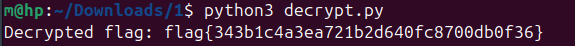
\includegraphics[width=1\linewidth]{static/solution_task_3}


    \section*{Task 4}
    \paragraph{Мейн}
Бинарный файл (ELF, x86\_64), в котором пользователь должен \("\)угадывать\("\) случайные числа.
\begin{verbatim}
        undefined8 FUN_00101200(void)

        {
          undefined *__s;
          uint in_EAX;
          time_t tVar1;
          long lVar2;
          size_t sVar3;
          int iVar4;
          int iVar5;
          int iVar6;
          ulong uVar7;
          undefined8 uStack_28;

          uStack_28 = (ulong)in_EAX;
          puts("Hello, You have to predict random numbers:");
          tVar1 = time((time_t *)0x0);
          srandom((uint)tVar1);
          iVar6 = 0x539;
          iVar5 = 0;
          do {
             __isoc99_scanf(&DAT_0010202b,(long)&uStack_28 + 4);
             lVar2 = random();
             __s = PTR_DAT_00104068;
             iVar4 = iVar5 + (uint)(lVar2 % 2 == (long)uStack_28._4_4_) * 2;
             iVar5 = iVar4 + -1;
             iVar6 = iVar6 + -1;
          } while (iVar6 != 0);
          if (iVar5 == 0x539) {
             if (*PTR_DAT_00104068 != '\0') {
                uVar7 = 0;
                do {
                  putchar((int)(char)__s[uVar7] ^ iVar4 - 0x52dU);
                  uVar7 = uVar7 + 1;
                  sVar3 = strlen(__s);
                } while (uVar7 < sVar3);
             }
          }
          else {
             printf("Oh noo ...");
          }
          return 0;
        }
\end{verbatim}

\paragraph{Описание}
\begin{itemize}
    \item Бинарный файл выводит: \("\)Hello, You have to predict random numbers:\("\)
    Затем вызывает \texttt{srandom(time(NULL))}, делая генератор случайных чисел предсказуемым, если известен момент запуска.

    \item Цикл длин ой 1337 итераций, где:
    \item Генерируется случайное число \texttt{random()}.
    \item Пользователь вводит 0 или 1 (угадывает чётность).
    \item Если угадывает — увеличивается счётчик.
    \item После 1337 правильных угадываний сравнивается результат:
    \item Если все угадывания верны — расшифровывается строка \texttt{PTR\_DAT\_00104068} с помощью XOR .
    \item XOR ключ вычисляется как \texttt{(iVar4 - 0x52d) = 1338--1325 = 13}.
\end{itemize}

Используя команду \texttt{strings task\_4} я получил что-то похожее на заiифрованный ключ: \texttt{kaljv44o<kk5k<<:5<89<k:k54k4oi9<n9l<:p}

Я создал питоновский скрипт, который использует библиотеки \texttt{random} для симуляции рандомного поведения кода
подбора букв и \texttt{time} для использования сида.
Далее скрипт дешифровывает с XOR ключом искомый флаг.
Найти скрипт можно по ссылке\cite{githublink}

\paragraph{Особенности}
\begin{itemize}
    \item Задача построена на использовании random() из glibc, который инициализируется с помощью srandom(time(NULL)).
    \item Это предсказуемо, если у нас есть примерное время запуска программы.
    \item Зашифрованный ключ: \texttt{kaljv44o<kk5k<<:5<89<k:k54k4oi9<n9l<:p}
    \item Дешифрованный ключ: \texttt{flag\{99b1ff8f11781541f7f89f9bd41c4a17\}}
\end{itemize}

\paragraph{Тестовый запуск}
Аутпут питоновского скрипта:

\paragraph{}
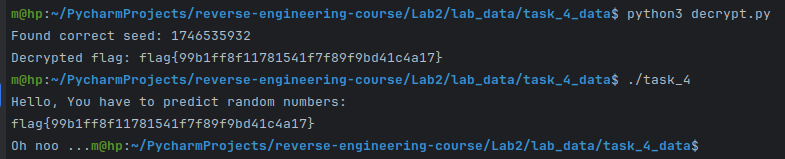
\includegraphics[width=1\linewidth]{static/solution_task_4}


    \section*{Task 5}
    \paragraph{Мейн}

Данный ELF исполняемый файл не запускался на моём компьютере из-за ошибок с библиотекой pyautogui и
отсутствия файла task\_4.py.
Для анализа использовался дизассемблер Ghidra.

\paragraph{Описание}
Программа task\_5 реализует загрузчик Python-приложения, упакованного с помощью PyInstaller.
Основная задача - извлечь необходимые файлы во временный каталог, настроить окружение Python и запустить приложение.

Ключевые компоненты и функциональность
\begin{itemize}
    \item Точка входа (processEntry)
    \begin{itemize}
        \item Вызывает \texttt{\_\_libc\_start\_main} для инициализации окружения.
        \item Передаёт управление основной функции \texttt{thunk\_FUN\_00403e50}
    \end{itemize}
    \item Основная функция \texttt{thunk\_FUN\_00403e50}
    \begin{itemize}
        \item Инициализация буферов и переменных
        \item Проверка переменных окружения:
        \begin{itemize}
            \item \texttt{\_MEIPASS2} - каталог с извлечёнными файлами
            \item \texttt{\_PYI\_ONEDIR\_MODE} - режим работы PyInstaller
            \item \texttt{\_PYI\_PROCNAME} - имя процесса Linux (устанавливается через prctl)
        \end{itemize}
    \end{itemize}
    \item Функция инициализации \texttt{FUN\_004086c0} - Конструктор, выполняющий \texttt{\_\_DT\_INIT\_ARRAY}
    до запуска основной функции
    \item Основные функции загрузчика
    \begin{itemize}
        \item Управление архивом PyInstaller
        \item Управление переменными окружения
        \item Обработка ошибок
        \item Управление памятью и очистка временных ресурсов
    \end{itemize}

\end{itemize}

\paragraph{Тестовый запуск}
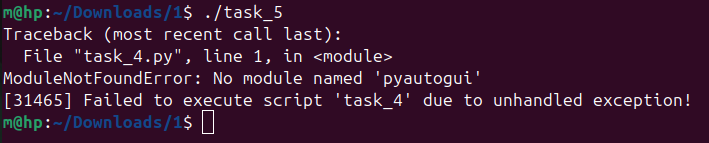
\includegraphics[width=1\linewidth]{static/_task_5}


    \section*{Task 6}
    \paragraph{Мейн информация}
Файл представляет собой ELF-бинарник под x86\_64 Linux.
При запуске программа предлагает пользователю выбрать один из двух режимов:
\begin{itemize}
    \item \textbf{1. Encrypton} --- зашифровать флаг из файла \texttt{flag.txt} и сохранить в \texttt{encrypted\_flag.txt}
    \item \textbf{2. Decryption} --- расшифровать содержимое \texttt{encrypted\_flag.txt} и сохранить в \texttt{flag.txt}
\end{itemize}

Вход обрабатывается функцией \texttt{FUN\_001011a0}, основной управляющей логикой занимается \texttt{FUN\_00101460}.

\paragraph{Анализ шифрования}

Функция шифрования представлена в дизассемблированном виде в \texttt{FUN\_00101280}.
Она применяет к каждому байту входной строки позиционно-зависимое преобразование.
Ниже приведена соответствующая формула:

\[
    \text{encrypted} = (i \oplus ((c - 0x19) \oplus \sim 0x28)) + 0x48
\]

где:
\begin{itemize}
    \item $c$ — ASCII-код исходного символа
    \item $i$ — индекс символа в строке
\end{itemize}

Пример кода на C (упрощённо):
\begin{verbatim}
        char c = input[i];
        char encrypted = (i ^ ((c - 0x19) ^ ~0x28)) + 0x48;
\end{verbatim}

Элементы шифра:
\begin{itemize}
    \item используется XOR с битовой маской
    \item учитывается позиция символа
    \item добавлены константные смещения (+0x19, +0x48 и др.)
\end{itemize}

\paragraph{Анализ дешифрования}

Дешифрование реализовано симметрично в \texttt{FUN\_00101380}.
Формула обратного преобразования выглядит так:

\[
    \text{original} = (((c - 0x29 - 0x1F) \oplus \sim 0x28) + 0x19) \oplus i
\]

Эквивалентный код на C:

\begin{verbatim}
        char c = input[i];
        char decrypted = (((c - 0x48) ^ ~0x28) + 0x19) ^ i;
\end{verbatim}

Зашифрованный флаг, прочитанный из файла, преобразуется обратно в оригинальную строку и сохраняется в \texttt{flag.txt}.

\paragraph{Особенности}

\begin{itemize}
    \item Используется самодельный криптоалгоритм с симметричным ключом.
    \item Преобразование для меня очень запутано, но линейно и обратимо.
    \item Для использования этого алгоритма обязательно использовать txt файлы для инпута и аутпута.
\end{itemize}

\paragraph{Тестовый запуск}

\paragraph{}
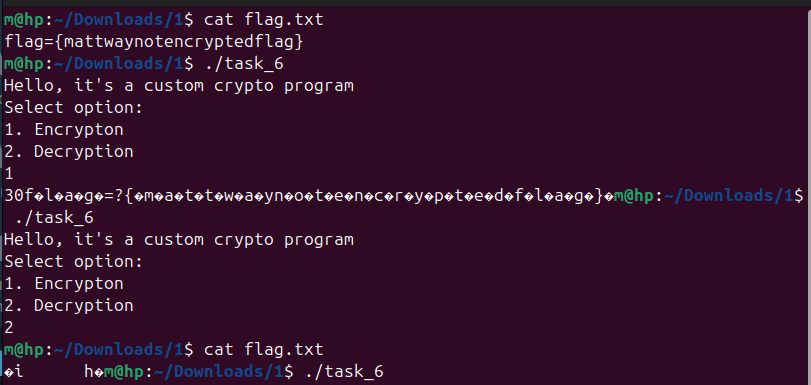
\includegraphics[width=1\linewidth]{static/_task_6}

Предполагаю, что я что-то сделал не так, поскольку формулы шифрации и дешифрации противопоставляют друг другу


    \section*{Task 7}
    \paragraph{Мейн информация}
Программа task\_7 является ELF исполняемым файлом.
Это текстовый энкодер, принимающий строку текста в качестве аргумента.

\paragraph{Описание}

\begin{itemize}
    \item Если программа запускается корректно, выполнение продолжается.
    \item Если программа запускается некорректно, выводится сообщение: "Usage: ./task\_7 TEXT"
    \item Программа выделяет память для локальных переменных.
    \item Для каждого символа входной строки выполняется последовательность операций:
    \begin{itemize}
        \item К символу добавляется его позиция в строке (ADD)
        \item Выполняется операция XOR с числом 14 (0xE)
        \item Применяется маска через AND с числом 31 (0x1F)
        \item Из результата вычитается (позиция + 1)
    \end{itemize}
    \item Результат выводится в консоль в виде бинарных данных.
\end{itemize}

\paragraph{Тестовый запуск}
Здесь я попробовал зашифровать фразу "Hello" и расшифровать ее с помощью дешифратора из 6й задачи, но ничего
не вышло(

\paragraph{}
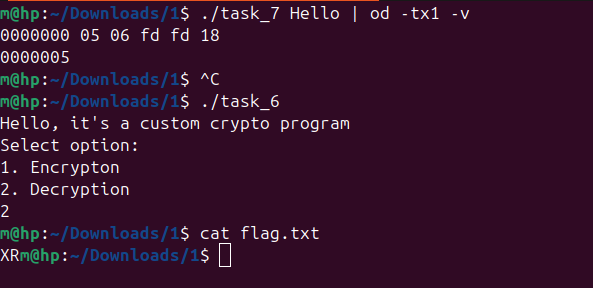
\includegraphics[width=1\linewidth]{static/_task_7}

Также я так и не нашел зависимость task\_2 от task\_7


    \section*{Task 8}
    \paragraph{Мейн информация}
Программа \texttt{task\_8} является исполняемым ELF-файлом.
Для анализа была рассмотрена функция входа, поскольку она вызывает множество других функций,
что затрудняет полное исследование всей программы.
На основе анализа можно предположить, что
\texttt{task\_8} является частью системного приложения или программного обеспечения,
связанного с обеспечением безопасности, учитывая наличие проверок, связанных с процессором.

\subsection*{2. Описание}
\subsubsection*{2.1 Проверка процессора}
Программа использует инструкцию \texttt{CPUID} для получения информации о процессоре.
В частности, при вызове с параметром \texttt{leaf = 0} вызывается функция \texttt{cpuid\_basic\_info(0)},
результат которой сохраняется в указатель \texttt{piVar1}.
Далее производится проверка идентификатора производителя процессора (vendor ID),
сопоставляя полученные значения с ожидаемыми константами:

\begin{itemize}
    \item 0x756e6547 (\texttt{"Genu"})
    \item 0x49656e69 (\texttt{"ineI"})
    \item 0x6c65746e (\texttt{"ntel"})
\end{itemize}

Если идентификатор совпадает с \texttt{"GenuineIntel"},
устанавливается флаг \texttt{DAT\_0054fea9 = 1}, сигнализирующий о том, что процессор Intel.

\subsubsection*{2.2 Получение версии процессора}
Далее программа вызывает \texttt{CPUID} с параметром \texttt{leaf = 1},
чтобы получить информацию о версии процессора через функцию \texttt{cpuid\_Version\_info(1)}.
Результат сохраняется в переменную \texttt{DAT\_0054ff04} для дальнейшего использования.

\subsubsection*{2.3 Логика инициализации}
Процесс инициализации программы разделяется в зависимости от значения указателя \texttt{DAT\_00520f48}:

\begin{itemize}
    \item Если \texttt{DAT\_00520f48 == NULL},
    выполняется инициализация с использованием ранее полученной информации о процессоре.
    В частности, производится проверка значения \texttt{0x123}.
    \item Если \texttt{DAT\_00520f48 != NULL}, происходит вызов функции через указатель с заданными параметрами,
    а также производится настройка смещений памяти.
\end{itemize}

\subsubsection*{2.4 Последовательные вызовы функций}

В завершении выполняются последовательные вызовы функций \texttt{FUN\_0045d1a0()}
и \texttt{FUN\_0045d160()}, которые делегируют выполнение функциям \texttt{FUN\_00440360()}
и \texttt{FUN\_0043fe80()} соответственно.
Эти функции включают:

\begin{itemize}
    \item Реализацию цикла, проверяющего состояние стека относительно \texttt{FS\_OFFSET}, для обеспечения целостности программы.
    \item Вызов функции \texttt{FUN\_00458c20()} в случае нарушения условия целостности.
    \item Манипуляции с глобальными переменными и условные вызовы дополнительных функций для настройки состояния программы.
    \item Последовательность проверок, операций с блокировками (\texttt{LOCK}/\texttt{UNLOCK}), изменяющих значения контрольных переменных.
    \item Многоступенчатую цепочку условий, включающую арифметические, побитовые и числовые проверки, а также обработку специальных случаев с использованием операций \texttt{NaN} для сравнения чисел с плавающей точкой.
    \item При определённых условиях происходит вызов \texttt{FUN\_00440160()}, \texttt{FUN\_0045ab60()} и \texttt{FUN\_0042fd40()} для завершения или корректировки работы программы.
    \item Функция \texttt{FUN\_00440160()} реализует цикл проверки адреса стека с вызовом \texttt{FUN\_00458c20()} при несоответствии, а также серию операций \texttt{LOCK}/\texttt{UNLOCK}, изменяющих глобальные переменные (например, \texttt{DAT\_00550080}, \texttt{DAT\_00550088}). Возвращаемое значение фиксировано (\texttt{0x2a}).
    \item Функция \texttt{FUN\_0045ab60()} представляет собой пустую функцию-заглушку (\texttt{return;}), возможно, зарезервированную для будущей логики или проверки наличия вызова.
    \item Функция \texttt{FUN\_0042fd40()} выполняет вызовы инициализации через \texttt{FUN\_00458ae0()} и \texttt{FUN\_0042ffa0()}, проверяет и устанавливает значение в структуре по смещению \texttt{0xf4}, а затем записывает значение 0 по адресу \texttt{uRam0000000000000000}.
\end{itemize}


\subsection*{3. Особенности}

\begin{itemize}

    \item Используется защита стека (через \texttt{in\_FS\_OFFSET}).
    \item Программа содержит структурированную обработку ошибок.
    \item Реализованы множественные проверки инициализации, обеспечивающие корректность запуска.
    \item Наблюдается сложная логика работы с глобальными переменными и флагами, а также использование атомарных операций для синхронизации.
    \item Программа реализует внутренние механизмы самопроверки и восстановления состояния при возникновении ошибок.
    \item Присутствуют функции-заглушки, не содержащие функциональной нагрузки, возможно,
    используемые как точки входа или метки для дальнейшего развития.
    \item Связь с task\_3 я также не нашел
\end{itemize}


    \begin{thebibliography}{1}
        \bibitem{githublink}
        GitHub Link: https://github.com/MattWay224/reverse-engineering-course
        В этом репозитории можно найти все лабы и информацию про каждое задание в каждой лабе
    \end{thebibliography}
\end{document}
